% Created by tikzDevice version 0.12.4 on 2023-02-28 04:54:11
% !TEX encoding = UTF-8 Unicode
\documentclass[tikz]{standalone}

\nonstopmode

\usepackage[fontset=fandol]{ctex}
\usepackage[default,semibold]{sourcesanspro}
\usepackage{amsfonts,mathrsfs,amssymb}
\begin{document}

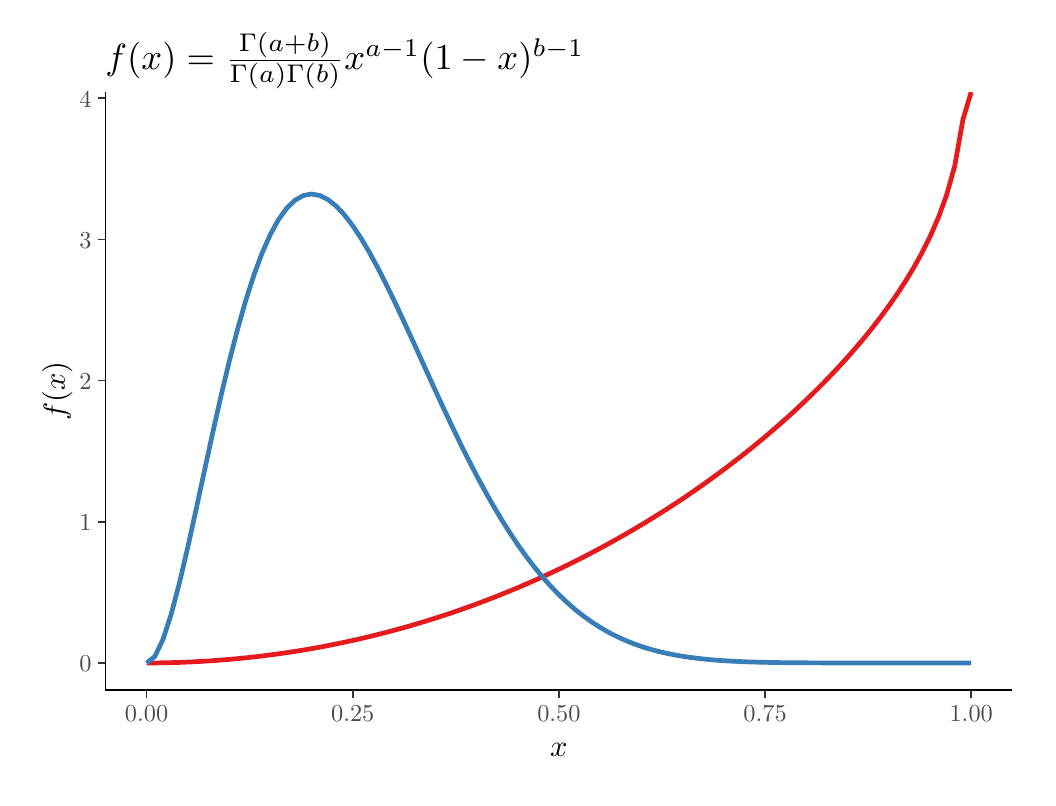
\begin{tikzpicture}[x=1pt,y=1pt]
\definecolor{fillColor}{RGB}{255,255,255}
\path[use as bounding box,fill=fillColor,fill opacity=0.00] (0,0) rectangle (361.35,271.01);
\begin{scope}
\path[clip] (  0.00,  0.00) rectangle (361.35,271.01);
\definecolor{drawColor}{RGB}{255,255,255}
\definecolor{fillColor}{RGB}{255,255,255}

\path[draw=drawColor,line width= 0.6pt,line join=round,line cap=round,fill=fillColor] (  0.00,  0.00) rectangle (361.35,271.01);
\end{scope}
\begin{scope}
\path[clip] ( 28.07, 31.63) rectangle (355.85,247.73);
\definecolor{fillColor}{RGB}{255,255,255}

\path[fill=fillColor] ( 28.07, 31.63) rectangle (355.85,247.73);
\definecolor{drawColor}{RGB}{228,26,28}

\path[draw=drawColor,line width= 1.7pt,line join=round] ( 42.97, 41.45) --
	( 45.95, 41.46) --
	( 48.93, 41.50) --
	( 51.91, 41.57) --
	( 54.89, 41.65) --
	( 57.87, 41.77) --
	( 60.85, 41.91) --
	( 63.83, 42.08) --
	( 66.81, 42.27) --
	( 69.79, 42.49) --
	( 72.77, 42.73) --
	( 75.75, 43.00) --
	( 78.73, 43.30) --
	( 81.71, 43.62) --
	( 84.69, 43.97) --
	( 87.67, 44.34) --
	( 90.65, 44.75) --
	( 93.63, 45.18) --
	( 96.61, 45.63) --
	( 99.59, 46.11) --
	(102.57, 46.62) --
	(105.55, 47.16) --
	(108.53, 47.73) --
	(111.51, 48.32) --
	(114.49, 48.94) --
	(117.47, 49.59) --
	(120.45, 50.26) --
	(123.43, 50.97) --
	(126.41, 51.70) --
	(129.39, 52.46) --
	(132.37, 53.25) --
	(135.35, 54.06) --
	(138.33, 54.91) --
	(141.31, 55.79) --
	(144.29, 56.69) --
	(147.27, 57.63) --
	(150.25, 58.59) --
	(153.23, 59.58) --
	(156.20, 60.61) --
	(159.18, 61.66) --
	(162.16, 62.75) --
	(165.14, 63.86) --
	(168.12, 65.01) --
	(171.10, 66.19) --
	(174.08, 67.40) --
	(177.06, 68.64) --
	(180.04, 69.91) --
	(183.02, 71.22) --
	(186.00, 72.56) --
	(188.98, 73.93) --
	(191.96, 75.34) --
	(194.94, 76.78) --
	(197.92, 78.25) --
	(200.90, 79.76) --
	(203.88, 81.31) --
	(206.86, 82.89) --
	(209.84, 84.51) --
	(212.82, 86.16) --
	(215.80, 87.85) --
	(218.78, 89.58) --
	(221.76, 91.35) --
	(224.74, 93.16) --
	(227.72, 95.01) --
	(230.70, 96.89) --
	(233.68, 98.83) --
	(236.66,100.80) --
	(239.64,102.82) --
	(242.62,104.88) --
	(245.60,106.99) --
	(248.58,109.15) --
	(251.56,111.35) --
	(254.54,113.61) --
	(257.52,115.91) --
	(260.50,118.28) --
	(263.48,120.69) --
	(266.46,123.17) --
	(269.44,125.71) --
	(272.42,128.31) --
	(275.40,130.97) --
	(278.38,133.71) --
	(281.36,136.53) --
	(284.34,139.42) --
	(287.32,142.40) --
	(290.29,145.47) --
	(293.27,148.64) --
	(296.25,151.91) --
	(299.23,155.31) --
	(302.21,158.84) --
	(305.19,162.52) --
	(308.17,166.37) --
	(311.15,170.42) --
	(314.13,174.69) --
	(317.11,179.25) --
	(320.09,184.16) --
	(323.07,189.51) --
	(326.05,195.46) --
	(329.03,202.27) --
	(332.01,210.42) --
	(334.99,221.06) --
	(337.97,237.90) --
	(340.95,247.73);
\definecolor{drawColor}{RGB}{55,126,184}

\path[draw=drawColor,line width= 1.7pt,line join=round] ( 42.97, 41.45) --
	( 45.95, 43.78) --
	( 48.93, 50.04) --
	( 51.91, 59.26) --
	( 54.89, 70.59) --
	( 57.87, 83.33) --
	( 60.85, 96.86) --
	( 63.83,110.68) --
	( 66.81,124.38) --
	( 69.79,137.62) --
	( 72.77,150.14) --
	( 75.75,161.71) --
	( 78.73,172.20) --
	( 81.71,181.50) --
	( 84.69,189.52) --
	( 87.67,196.25) --
	( 90.65,201.67) --
	( 93.63,205.79) --
	( 96.61,208.67) --
	( 99.59,210.35) --
	(102.57,210.89) --
	(105.55,210.37) --
	(108.53,208.88) --
	(111.51,206.50) --
	(114.49,203.32) --
	(117.47,199.43) --
	(120.45,194.92) --
	(123.43,189.89) --
	(126.41,184.41) --
	(129.39,178.57) --
	(132.37,172.45) --
	(135.35,166.12) --
	(138.33,159.65) --
	(141.31,153.10) --
	(144.29,146.54) --
	(147.27,140.00) --
	(150.25,133.55) --
	(153.23,127.23) --
	(156.20,121.05) --
	(159.18,115.07) --
	(162.16,109.30) --
	(165.14,103.77) --
	(168.12, 98.49) --
	(171.10, 93.47) --
	(174.08, 88.73) --
	(177.06, 84.26) --
	(180.04, 80.08) --
	(183.02, 76.18) --
	(186.00, 72.55) --
	(188.98, 69.20) --
	(191.96, 66.11) --
	(194.94, 63.28) --
	(197.92, 60.69) --
	(200.90, 58.34) --
	(203.88, 56.21) --
	(206.86, 54.29) --
	(209.84, 52.57) --
	(212.82, 51.04) --
	(215.80, 49.68) --
	(218.78, 48.47) --
	(221.76, 47.41) --
	(224.74, 46.48) --
	(227.72, 45.67) --
	(230.70, 44.97) --
	(233.68, 44.37) --
	(236.66, 43.85) --
	(239.64, 43.42) --
	(242.62, 43.05) --
	(245.60, 42.74) --
	(248.58, 42.48) --
	(251.56, 42.26) --
	(254.54, 42.09) --
	(257.52, 41.95) --
	(260.50, 41.83) --
	(263.48, 41.74) --
	(266.46, 41.67) --
	(269.44, 41.61) --
	(272.42, 41.57) --
	(275.40, 41.54) --
	(278.38, 41.51) --
	(281.36, 41.49) --
	(284.34, 41.48) --
	(287.32, 41.47) --
	(290.29, 41.46) --
	(293.27, 41.46) --
	(296.25, 41.46) --
	(299.23, 41.45) --
	(302.21, 41.45) --
	(305.19, 41.45) --
	(308.17, 41.45) --
	(311.15, 41.45) --
	(314.13, 41.45) --
	(317.11, 41.45) --
	(320.09, 41.45) --
	(323.07, 41.45) --
	(326.05, 41.45) --
	(329.03, 41.45) --
	(332.01, 41.45) --
	(334.99, 41.45) --
	(337.97, 41.45) --
	(340.95, 41.45);
\end{scope}
\begin{scope}
\path[clip] (  0.00,  0.00) rectangle (361.35,271.01);
\definecolor{drawColor}{RGB}{0,0,0}

\path[draw=drawColor,line width= 0.6pt,line join=round] ( 28.07, 31.63) --
	( 28.07,247.73);
\end{scope}
\begin{scope}
\path[clip] (  0.00,  0.00) rectangle (361.35,271.01);
\definecolor{drawColor}{gray}{0.30}

\node[text=drawColor,anchor=base east,inner sep=0pt, outer sep=0pt, scale=  0.88] at ( 23.12, 38.26) {0};

\node[text=drawColor,anchor=base east,inner sep=0pt, outer sep=0pt, scale=  0.88] at ( 23.12, 89.26) {1};

\node[text=drawColor,anchor=base east,inner sep=0pt, outer sep=0pt, scale=  0.88] at ( 23.12,140.27) {2};

\node[text=drawColor,anchor=base east,inner sep=0pt, outer sep=0pt, scale=  0.88] at ( 23.12,191.28) {3};

\node[text=drawColor,anchor=base east,inner sep=0pt, outer sep=0pt, scale=  0.88] at ( 23.12,242.28) {4};
\end{scope}
\begin{scope}
\path[clip] (  0.00,  0.00) rectangle (361.35,271.01);
\definecolor{drawColor}{gray}{0.20}

\path[draw=drawColor,line width= 0.6pt,line join=round] ( 25.32, 41.45) --
	( 28.07, 41.45);

\path[draw=drawColor,line width= 0.6pt,line join=round] ( 25.32, 92.46) --
	( 28.07, 92.46);

\path[draw=drawColor,line width= 0.6pt,line join=round] ( 25.32,143.46) --
	( 28.07,143.46);

\path[draw=drawColor,line width= 0.6pt,line join=round] ( 25.32,194.47) --
	( 28.07,194.47);

\path[draw=drawColor,line width= 0.6pt,line join=round] ( 25.32,245.48) --
	( 28.07,245.48);
\end{scope}
\begin{scope}
\path[clip] (  0.00,  0.00) rectangle (361.35,271.01);
\definecolor{drawColor}{RGB}{0,0,0}

\path[draw=drawColor,line width= 0.6pt,line join=round] ( 28.07, 31.63) --
	(355.85, 31.63);
\end{scope}
\begin{scope}
\path[clip] (  0.00,  0.00) rectangle (361.35,271.01);
\definecolor{drawColor}{gray}{0.20}

\path[draw=drawColor,line width= 0.6pt,line join=round] ( 42.97, 28.88) --
	( 42.97, 31.63);

\path[draw=drawColor,line width= 0.6pt,line join=round] (117.47, 28.88) --
	(117.47, 31.63);

\path[draw=drawColor,line width= 0.6pt,line join=round] (191.96, 28.88) --
	(191.96, 31.63);

\path[draw=drawColor,line width= 0.6pt,line join=round] (266.46, 28.88) --
	(266.46, 31.63);

\path[draw=drawColor,line width= 0.6pt,line join=round] (340.95, 28.88) --
	(340.95, 31.63);
\end{scope}
\begin{scope}
\path[clip] (  0.00,  0.00) rectangle (361.35,271.01);
\definecolor{drawColor}{gray}{0.30}

\node[text=drawColor,anchor=base,inner sep=0pt, outer sep=0pt, scale=  0.88] at ( 42.97, 20.29) {0.00};

\node[text=drawColor,anchor=base,inner sep=0pt, outer sep=0pt, scale=  0.88] at (117.47, 20.29) {0.25};

\node[text=drawColor,anchor=base,inner sep=0pt, outer sep=0pt, scale=  0.88] at (191.96, 20.29) {0.50};

\node[text=drawColor,anchor=base,inner sep=0pt, outer sep=0pt, scale=  0.88] at (266.46, 20.29) {0.75};

\node[text=drawColor,anchor=base,inner sep=0pt, outer sep=0pt, scale=  0.88] at (340.95, 20.29) {1.00};
\end{scope}
\begin{scope}
\path[clip] (  0.00,  0.00) rectangle (361.35,271.01);
\definecolor{drawColor}{RGB}{0,0,0}

\node[text=drawColor,anchor=base,inner sep=0pt, outer sep=0pt, scale=  1.10] at (191.96,  7.75) {$x$};
\end{scope}
\begin{scope}
\path[clip] (  0.00,  0.00) rectangle (361.35,271.01);
\definecolor{drawColor}{RGB}{0,0,0}

\node[text=drawColor,rotate= 90.00,anchor=base,inner sep=0pt, outer sep=0pt, scale=  1.10] at ( 13.48,139.68) {$f(x)$};
\end{scope}
\begin{scope}
\path[clip] (  0.00,  0.00) rectangle (361.35,271.01);
\definecolor{drawColor}{RGB}{0,0,0}

\node[text=drawColor,anchor=base west,inner sep=0pt, outer sep=0pt, scale=  1.32] at ( 28.07,255.93) {$f(x) = \frac{\Gamma(a+b)}{\Gamma(a)\Gamma(b)}x^{a-1}(1-x)^{b-1}$};
\end{scope}
\end{tikzpicture}

\end{document}
